\documentclass{ML}

% 姓名,学号
\infoauthor{朱明彦}{1160300314}

% 课程类型,实验名称
\infoexp{课程类型}{实验二}

\infoschool{计算机学院}{高宏}

\begin{document}
\maketitle

\tableofcontents
\newpage

\begin{center}
    \textbf{\zihao{3} 实验二 \ 使用高级语言操作MySQL数据库}
\end{center}
% 对于 3.1,粘贴 9 条 sql 语句的核心高级语言函数代码以及相应的查询结果,
% 作为评分标准。先进行 3.2-3.5 的操作练习,结果无需截图。
\section{实验目的}
学会使用高级语言访问 MySQL 数据库,并进行查询。
\section{实验环境}
\begin{itemize}
    \item Ubuntu 16.04.5; MySQL Ver 14.14 Distrib 5.7.25
    % \item MySQL Ver 14.14 Distrib 5.7.25
    \item Java version 1.8.0\_181; IDEA 2018.3.5
    % \item IntelliJ IDEA Ultimate 2018.3.5
\end{itemize}
\section{实验过程及结果}
实验中统一使用的命令行语句如下所示
\begin{minted}{shell}
    java -cp /lib/java_lib/commons-cli-1.4.jar:\
    /lib/java_lib/mysql-connector-java-5.1.47.jar:\ 
    COMPANY_Query -q <Number> -p [Parameters]
\end{minted}
\begin{enumerate}
    \item \begin{minted}{Java}
    String PARA_PNO = "%PNO%";
    String query = "SELECT ESSN FROM WORKS_ON 
                        WHERE PNO = \"" + PARA_PNO + "\"";
    System.out.println("Query " + count);
    System.out.println("Please input pno:");
    String pno = cin.nextLine();
    query = query.replace(PARA_PNO, pno);
    resultSet = statement.executeQuery(query);
    System.out.println("ESSN");
    while (resultSet.next())
        System.out.println(resultSet.getNString("ESSN"));
    \end{minted}
    当输入\texttt{\%PNO\%}为\texttt{P1}时, 实验结果如图\ref{fig:3.1}所示,由于结果过长,此处仅仅截取了部分结果。
    \begin{figure}[H]
        \centering
        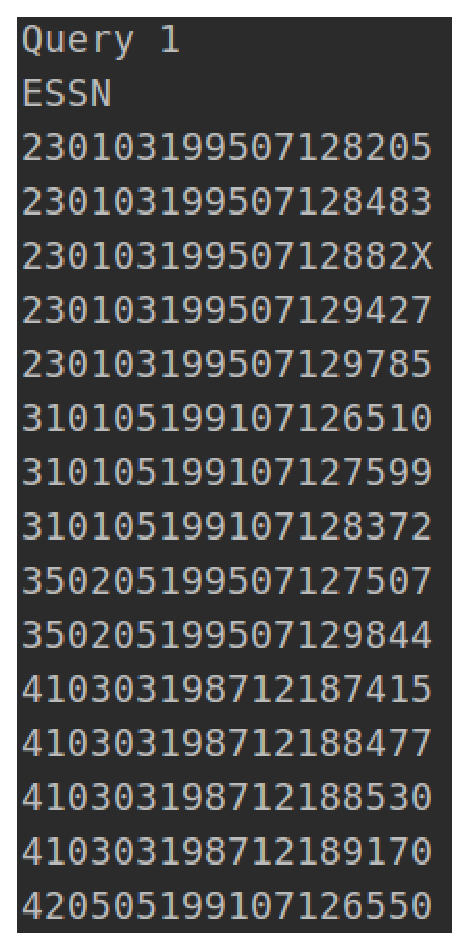
\includegraphics[scale=0.4, bb=0 0 209 440]{media/3.1.eps}
        \caption{参加了项目编号为 \texttt{\%PNO\%} 的项目的员工姓名}\label{fig:3.1}
    \end{figure}
   \item \begin{minted}{Java}
    String PARA_PNAME = "%PNAME%";
    String query = "SELECT ENAME FROM EMPLOYEE, WORKS_ON, PROJECT 
                    WHERE EMPLOYEE.ESSN = WORKS_ON.ESSN 
                        AND PROJECT.PNO = WORKS_ON.PNO 
                        AND PROJECT.PNAME = \"" + PARA_PNAME + "\"";
    System.out.println("Query " + count);
    System.out.println("Please input pname:");
    String pname = cin.nextLine();
    query = query.replace(PARA_PNAME, pname);
    resultSet = statement.executeQuery(query);
    System.out.println("ENAME");
    while (resultSet.next())
        System.out.println(resultSet.getNString("ENAME"));
    \end{minted}
    当输入\texttt{\%PNAME\%}为\texttt{SQL Project}时, 实验结果如图\ref{fig:3.2}所示.
    \begin{figure}[H]
        \centering
        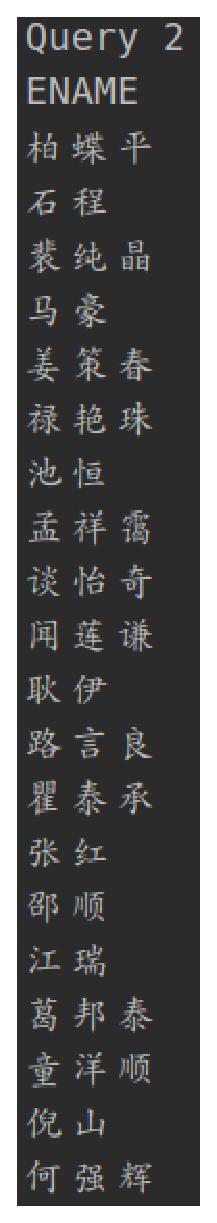
\includegraphics[scale = 0.5, bb= 0 0 88 571]{media/3.2.eps}
        \caption{参加了项目名为\texttt{\%PNAME\%}的员工名字}\label{fig:3.2}
    \end{figure}
    \item \begin{minted}{Java}
    String PARA_DNAME = "%DNAME%";
    String query = "SELECT ENAME, ADDRESS FROM EMPLOYEE, DEPARTMENT 
                    WHERE EMPLOYEE.DNO = DEPARTMENT.DNO 
                        AND DEPARTMENT.DNAME = \"";
    System.out.println("Query " + count);
    System.out.println("Please input dname:");
    String dname = cin.nextLine();
    query = query.replace(PARA_DNAME, dname);
    resultSet = statement.executeQuery(query);
    System.out.println("ENAME");
    while (resultSet.next())
        System.out.println(resultSet.getNString("ENAME") + 
                            "\t" + resultSet.getNString("ADDRESS"));
    \end{minted}
    当输入\texttt{\%DNAME\%}为\texttt{International Department}时, 实验结果如图\ref{fig:3.3}所示.
    \begin{figure}[H]
        \centering
        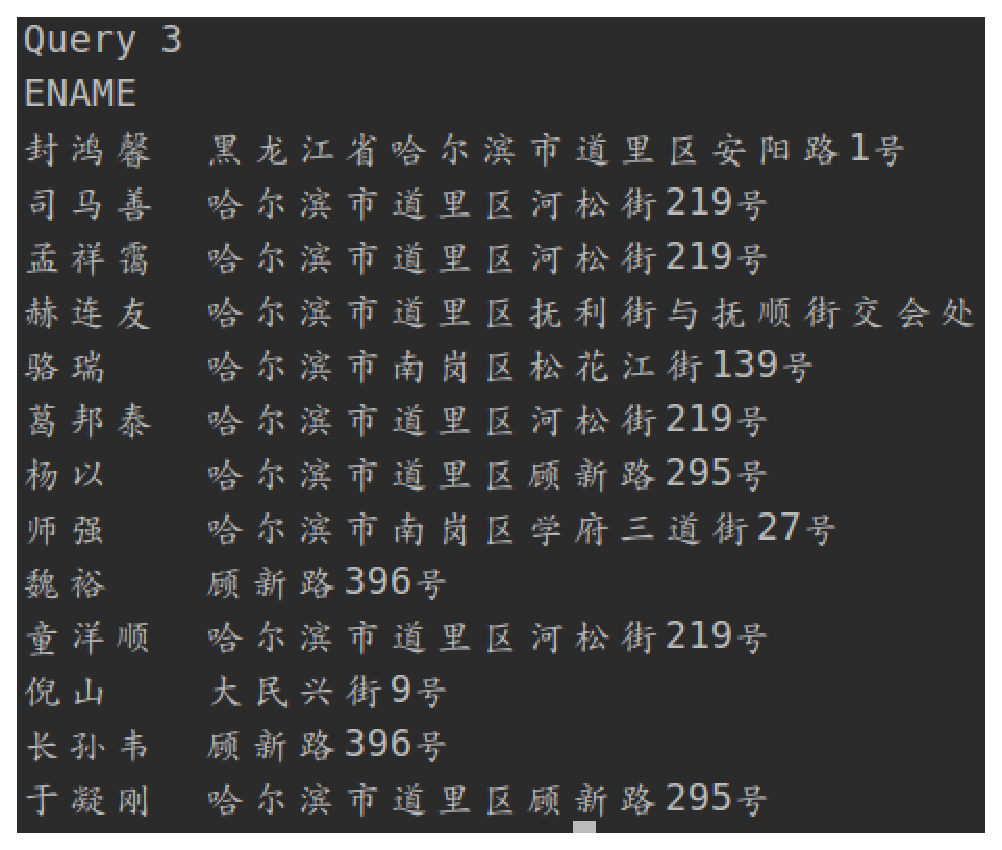
\includegraphics[scale = 0.5, bb= 0 0 465 392]{media/3.3.eps}
        \caption{在\texttt{\%PNAME\%}工作的所有工作人员的名字和地址}\label{fig:3.3}
    \end{figure}
    \item \begin{minted}{Java}
    String PARA_SALARY = "%SALARY%";
    String PARA_DNAME = "%DNAME%";
    String query = "SELECT ENAME, ADDRESS FROM EMPLOYEE, DEPARTMENT 
                    WHERE EMPLOYEE.DNO = DEPARTMENT.DNO 
                        AND DEPARTMENT.DNAME = \"" + PARA_DNAME + "\" 
                        AND SALARY < " + PARA_SALARY;
    System.out.println("Query " + count);
    System.out.println("Please input dname:");
    dname = cin.nextLine();
    System.out.println("Please input salary:");
    int salary = Integer.parseInt(cin.nextLine());
    query = query.replace(PARA_DNAME, dname)
                 .replace(PARA_SALARY, String.valueOf(salary));
    resultSet = statement.executeQuery(query);
    System.out.println("ENAME\tADDRESS");
    while (resultSet.next())
        System.out.println(resultSet.getNString("ENAME") + 
                            "\t" + resultSet.getNString("ADDRESS"));

    \end{minted}
    当输入\texttt{\%DNAME\%}为\texttt{International Department}, 输入\texttt{\%SALARY\%}为\texttt{4000}时, 实验结果如图\ref{fig:3.4}所示.
    \begin{figure}[H]
        \centering
        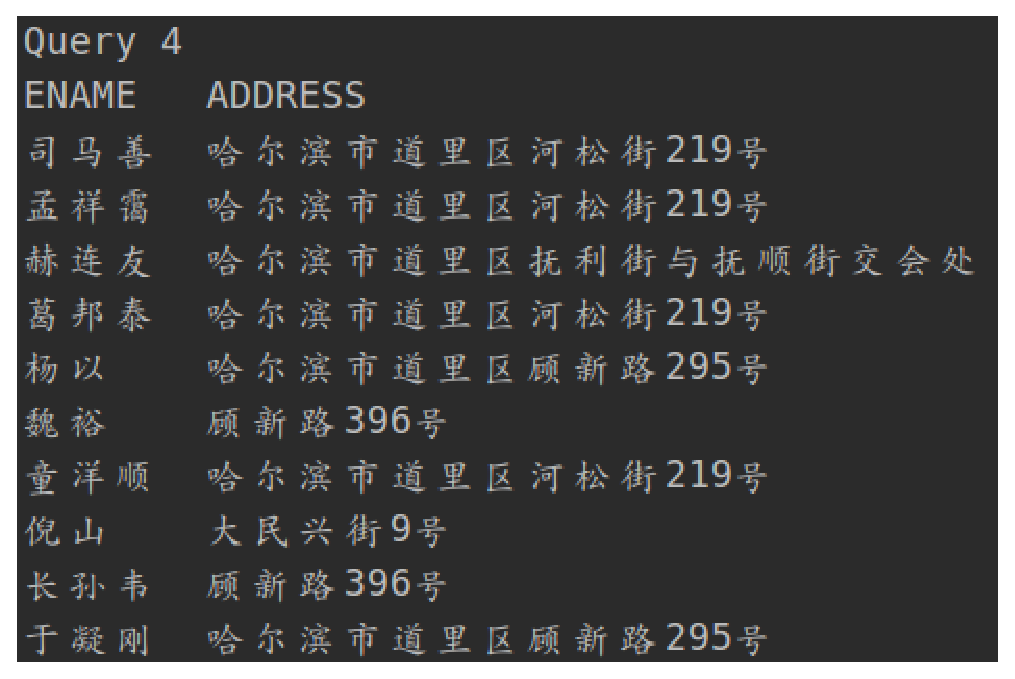
\includegraphics[scale = 0.5, bb= 0 0 471 310]{media/3.4.eps}
        \caption{在\texttt{\%DNAME\%}工作且工资低于\texttt{\%SALARY\%}的员工的名字和地址}\label{fig:3.4}
    \end{figure}
    \item \begin{minted}{Java}
        String PARA_PNO = "%PNO%";
        String query = "SELECT ENAME FROM EMPLOYEE 
        WHERE ESSN NOT IN (
            SELECT DISTINCT ESSN 
            FROM WORKS_ON 
            WHERE WORKS_ON.PNO =\"" + PARA_PNO + "\")";
            System.out.println("Query " + count);
            System.out.println("Please input pno");
            pno = cin.nextLine();
            query = query.replace(PARA_PNO, pno);
            resultSet = statement.executeQuery(query);
            System.out.println("ENAME");
            while (resultSet.next())
                System.out.println(resultSet.getNString("ENAME"));
        \end{minted}
    当输入\texttt{\%PNO\%}为\texttt{P2}时, 实验结果如图\ref{fig:3.5}所示.
    \begin{figure}[H]
        \centering
        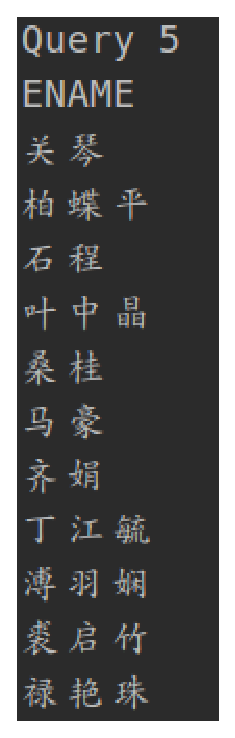
\includegraphics[scale=0.4, bb=0 0 97 338]{media/3.5.eps}
        \caption{没有参加项目编号为\texttt{\%PNO\%}的项目的员工姓名}\label{fig:3.5}
    \end{figure}
    \item \begin{minted}{Java}
    String PARA_ENAME = "%ENAME%";
    String query = "SELECT ENAME, DNAME FROM EMPLOYEE, DEPARTMENT 
                    WHERE EMPLOYEE.DNO = DEPARTMENT.DNO 
                    AND EMPLOYEE.SUPERSSN IN (
                        SELECT ESSN FROM EMPLOYEE 
                        WHERE ENAME = \"" + PARA_ENAME + "\")";
    System.out.println("Query " + count);
    System.out.println("Please input ename");
    String ename = cin.nextLine();
    query = query.replace(PARA_ENAME, ename);
    resultSet = statement.executeQuery(query);
    System.out.println("ENAME\tDNAME");
    while (resultSet.next())
        System.out.println(resultSet.getNString("ENAME") + 
                            "\t" + resultSet.getNString("DNAME"));
    \end{minted}
    当输入\texttt{\%ENAME\%}为\texttt{张红}时, 实验结果如图\ref{fig:3.6}所示.
    \begin{figure}[H]
        \centering
        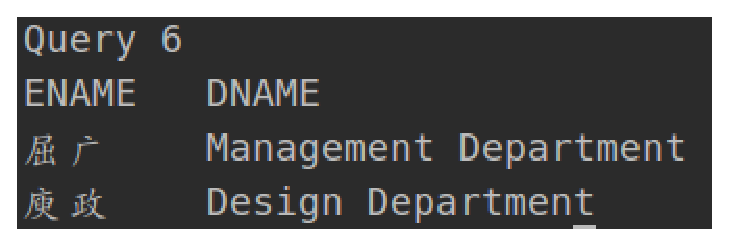
\includegraphics[scale=0.5, bb = 0 0 334 102]{media/3.6.eps}
        \caption{由\texttt{\%ENAME\%}领导的工作人员的姓名和所在的部门名字}\label{fig:3.6}
    \end{figure}
    \item \begin{minted}{Java}
    String PARA_PNO = "%PNO%";
    String query = "SELECT ESSN FROM WORKS_ON 
                    WHERE PNO = \"" + PARA_PNO + "1\" 
                    AND ESSN IN (
                        SELECT ESSN FROM WORKS_ON 
                        WHERE PNO = \"" + PARA_PNO + "2\")";
    System.out.println("Query " + count);
    System.out.println("Please input pno1");
    pno = cin.nextLine();
    query = query.replace(PARA_PNO+1, pno);
    System.out.println("Please input pno2");
    pno = cin.nextLine();
    query = query.replace(PARA_PNO+2, pno);
    resultSet = statement.executeQuery(query);
    System.out.println("ESSN");
    while (resultSet.next())
        System.out.println(resultSet.getNString("ESSN"));
    \end{minted}
    当输入\texttt{\%PNO1\%}为\texttt{P1}, \texttt{\%PNO\%}为\texttt{P2}时, 实验结果如图\ref{fig:3.7}所示.
    \begin{figure}[H]
        \centering
        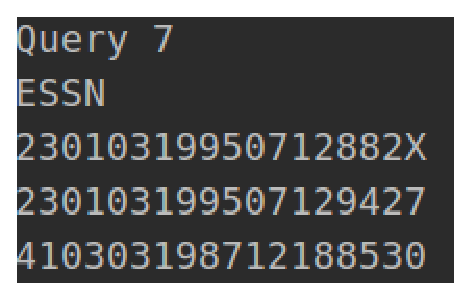
\includegraphics[scale = 0.5, bb = 0 0 210 128]{media/3.7.eps}
        \caption{至少参加了项目编号为\texttt{\%PNO1\%}和\texttt{\%PNO2\%}的项目的员工号}\label{fig:3.7}
    \end{figure}
    \item \begin{minted}{Java}
    String PARA_SALARY = "%SALARY%";
    String query = "SELECT DNAME FROM EMPLOYEE, DEPARTMENT 
                    WHERE EMPLOYEE.DNO = DEPARTMENT.DNO 
                    GROUP BY DEPARTMENT.DNO 
                    HAVING AVG(SALARY) < " + PARA_SALARY;
    System.out.println("Query " + count);
    System.out.println("Please input salary:");
    salary = Integer.parseInt(cin.nextLine());
    query = query.replace(PARA_SALARY, String.valueOf(salary));
    resultSet = statement.executeQuery(query);
    System.out.println("DNAME");
    while (resultSet.next())
        System.out.println(resultSet.getNString("DNAME"));
    \end{minted}
    当输入\texttt{\%SALARY\%}为\texttt{3000}时, 实验结果如图\ref{fig:3.8}所示.
    \begin{figure}[H]
    \centering
    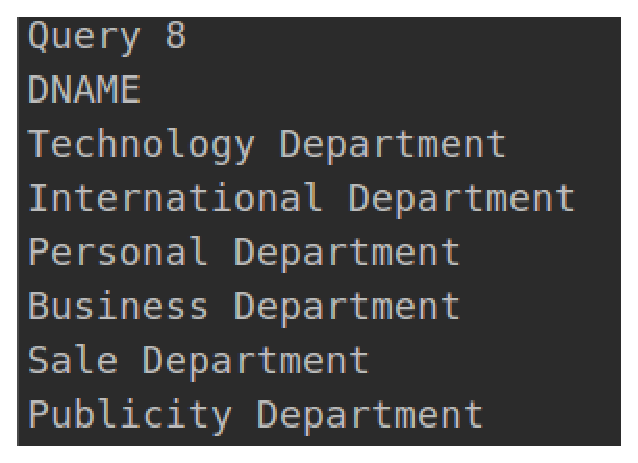
\includegraphics[scale=0.5, bb=0 0 290 206]{media/3.8.eps}
    \caption{员工平均工资低于\texttt{\%SALARY\%}元的部门名称}\label{fig:3.8}
    \end{figure}
    \item \begin{minted}{Java}
    String PARA_N = "%N%";
    String PARA_HOURS = "%HOURS%";
    String query = "SELECT ENAME FROM EMPLOYEE, WORKS_ON 
                    WHERE EMPLOYEE.ESSN = WORKS_ON.ESSN 
                    GROUP BY EMPLOYEE.ESSN 
                    HAVING COUNT(PNO) >= " + PARA_N + " 
                        AND SUM(HOURS) <= " + PARA_HOURS;    ;
    System.out.println("Query " + count);
    System.out.println("Please input n:");
    int n = Integer.parseInt(cin.nextLine());
    query = query.replace(PARA_N, String.valueOf(n));
    System.out.println("Please input hours:");
    int hours = Integer.parseInt(cin.nextLine());
    query = query.replace(PARA_HOURS, String.valueOf(hours));
    resultSet = statement.executeQuery(query);
    System.out.println("ENAME");
    while (resultSet.next())
        System.out.println(resultSet.getNString("ENAME"));
    \end{minted}
    当输入\texttt{\%N\%}为\texttt{3}, 输入\texttt{\%HOURS\%}为\texttt{8}时, 实验结果如图\ref{fig:3.9}所示.
    \begin{figure}[H]
        \centering
        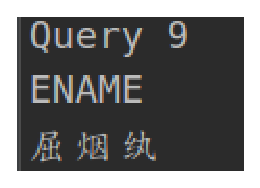
\includegraphics[scale = 0.5, bb=0 0 109 74]{media/3.9.eps}
        \caption{至少参加了\texttt{\%N\%}个项目且工作总时间不超过\texttt{\%HOURS\%}小时的员工名字}\label{fig:3.9}
    \end{figure}
\end{enumerate}
\section{实验心得}
本次实验可以选择使用不同的高级语言来完成, 此处用JAVA来完成实验, 相比使用C连接数据库, 仅仅需要将相应的\texttt{jar}包导入即可.
总的来说, 实验的难度不大.
% \appendix

% \section{源代码}
% \section{参考文献}
% \begin{thebibliography}{20}
%     % \bibitem{employee_name} 中国最常见名字前50名, \texttt{https://www.sohu.com/a/164406113\_367620}
%     \bibitem{employee_id} 身份证号在线生成器, \texttt{https://www.tinysoft.org/}
% \end{thebibliography}

\end{document}
